\chapter{Oracle Aplication Express}

\section{Tahapan Penggunaan Aplikasi Oracle Apex}
Langkah pertama yang harus dilakukan adalah membuka website https://apex.oracle.com, disini kita akan mendapatkan akses untuk memasuki Oracle Apllication Express, pastikan email yang dimasukkan valid untuk membuat Workspace, berikut adalah langkah langkah pembuatan Aplikasi pada Oracle APEX :

\begin{enumerate}
\item[1]Pergi ke Website Oracle APEX, https://apex.oracle.com, lalu klik Sign In.
\begin{figure}[!htbp]
    \begin{center}
    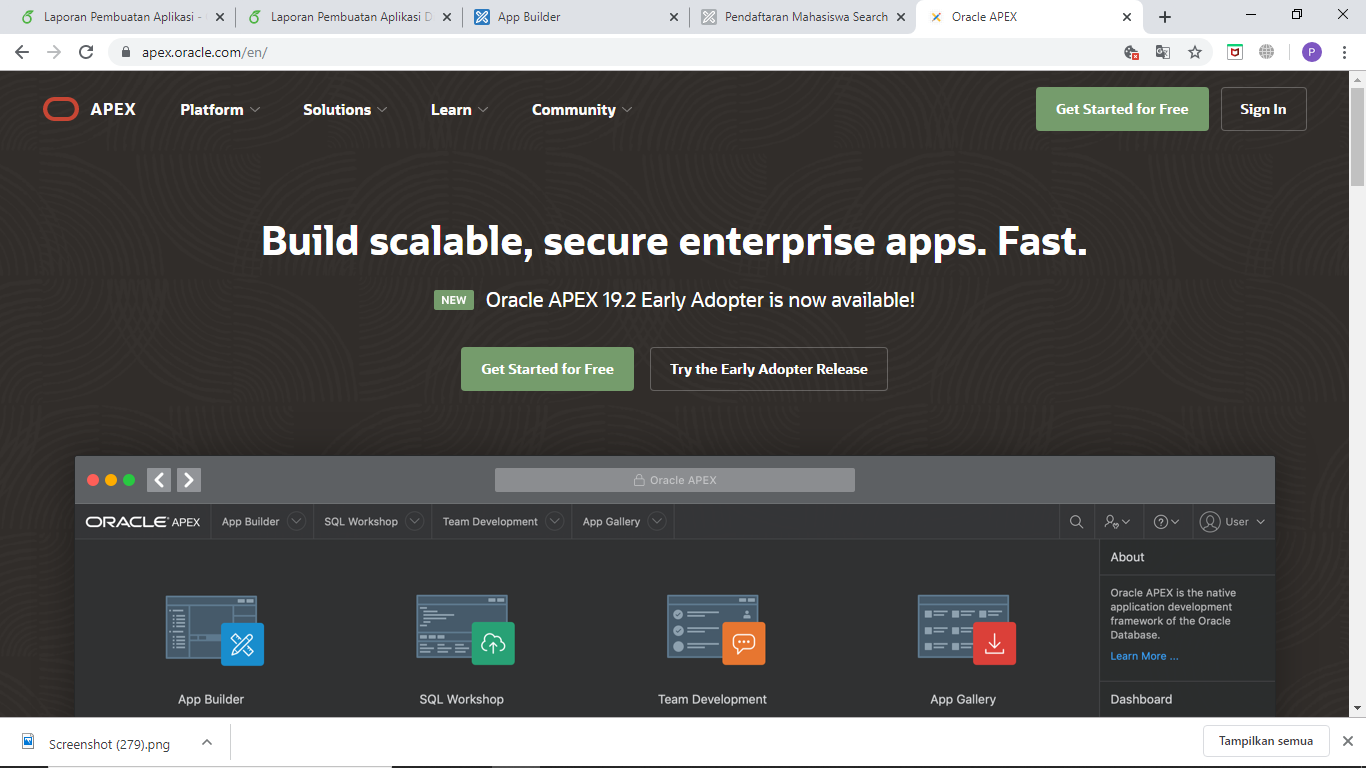
\includegraphics[scale=0.2]{figures/14.png}
    \caption{\textit{Sign In.}}
    \end{center}   
\end{figure} 
   
\begin{figure}[!htbp]
\item[2]Masukan Workspace yang telah dibuat, jika belum klik Request a Workspace.
    \begin{center}
    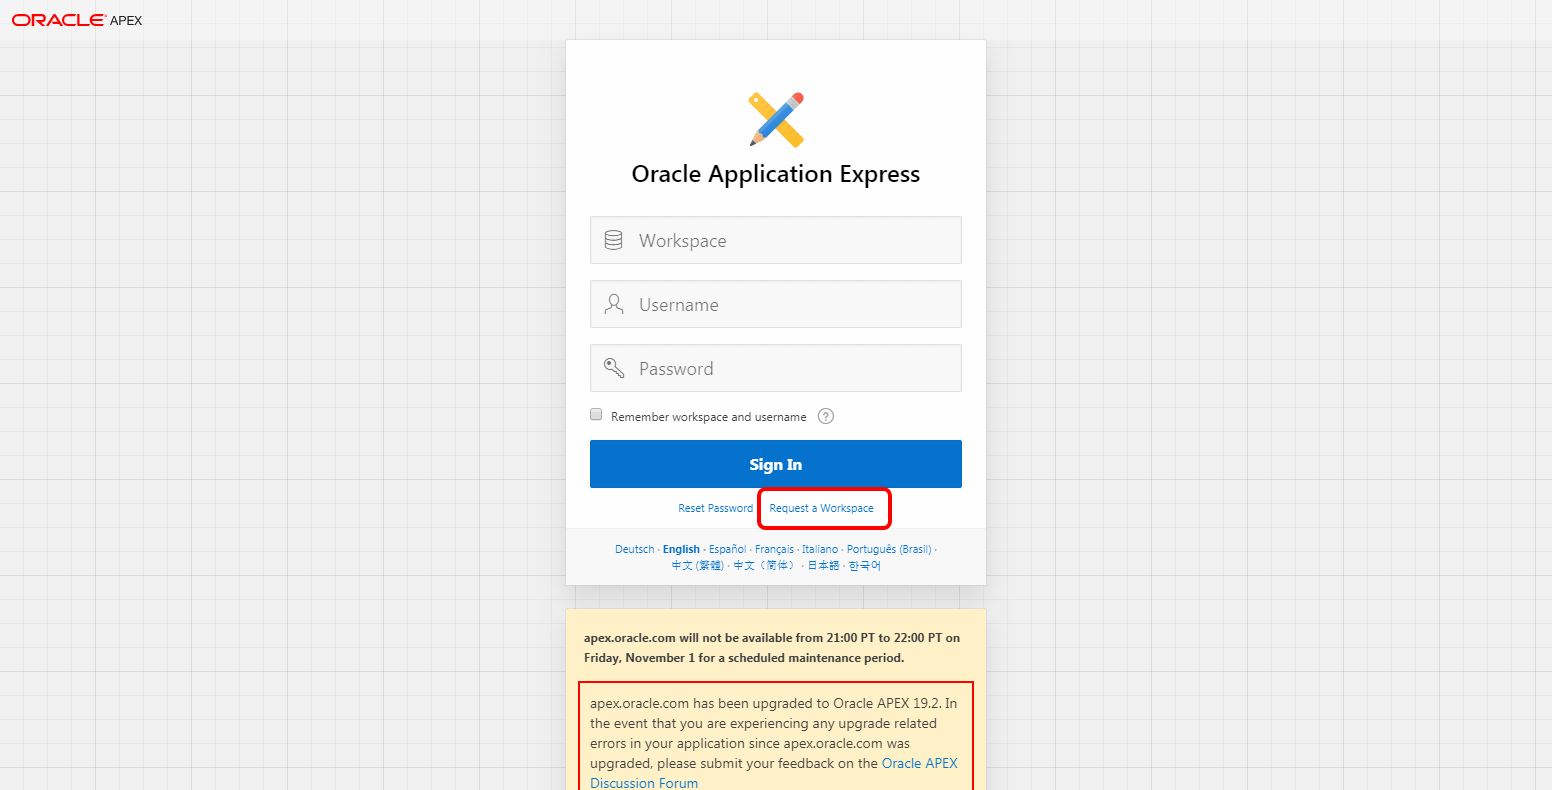
\includegraphics[scale=0.2]{figures/tahap1.png}
    \caption{\textit{Tahapan pembuatan Workspace.}}
    \end{center}
\end{figure}

\begin{figure}[!htbp]
\item[3] Setelah itu wajib isikan fist name, last name, email, dan workspace
	\begin{center}
	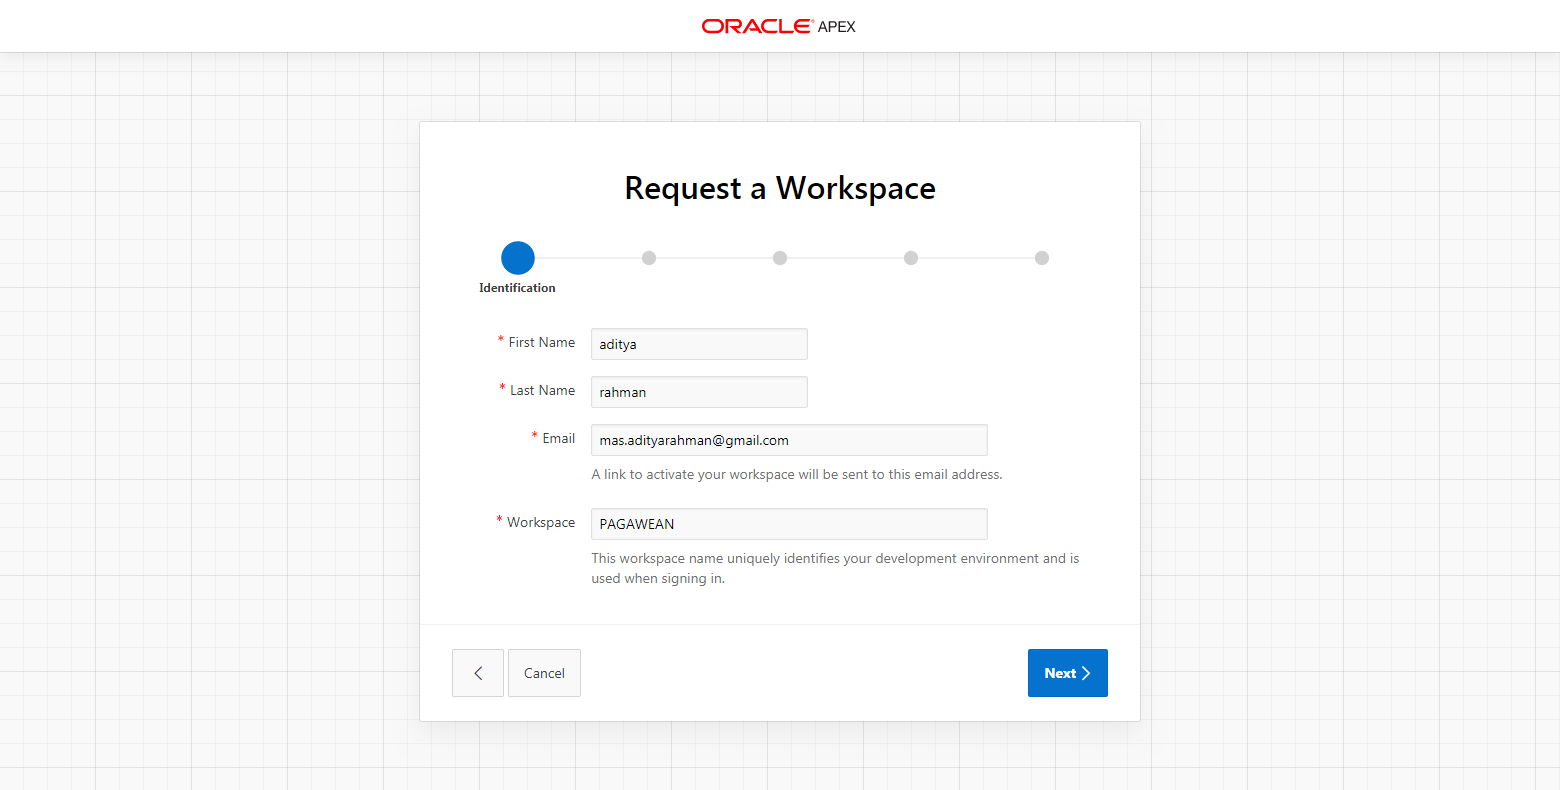
\includegraphics[scale=0.2]{figures/tahap2.png}
    \caption{\textit{Isi nama Request a Workspace}}
    \end{center}
\end{figure}

\begin{figure}[!htbp]
\item[4] Isi kalimat pertanyaan sebagai berikut.
	\begin{center}
	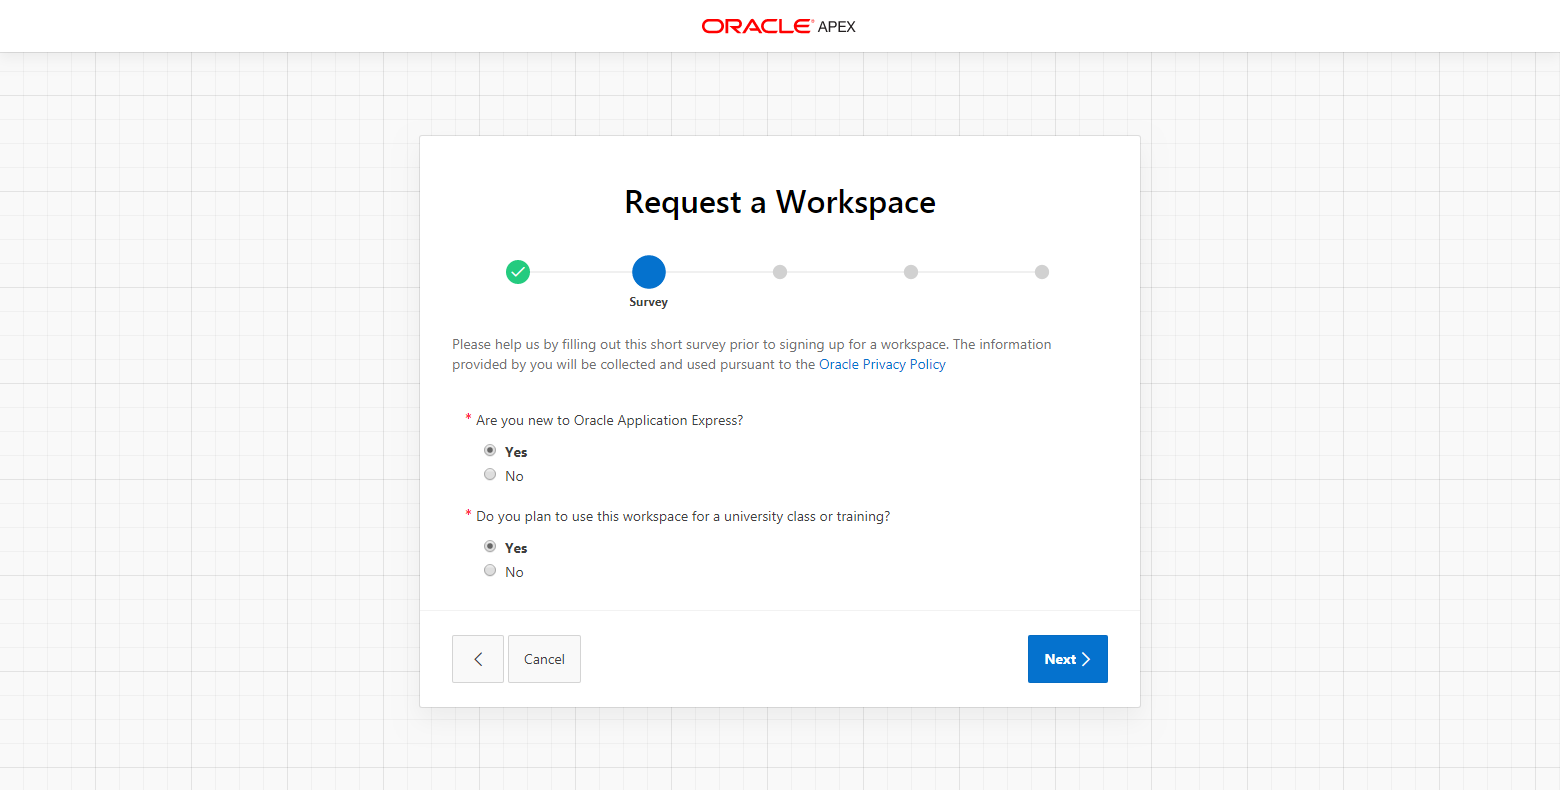
\includegraphics[scale=0.2]{figures/tahap3.png}
	\caption{\textit{Jawab pertanyaan}}
	\end{center}	 
\end{figure}

\begin{figure}[!htbp]
\item[5] Maka setelah itu isi kan justification.
	\begin{center}
	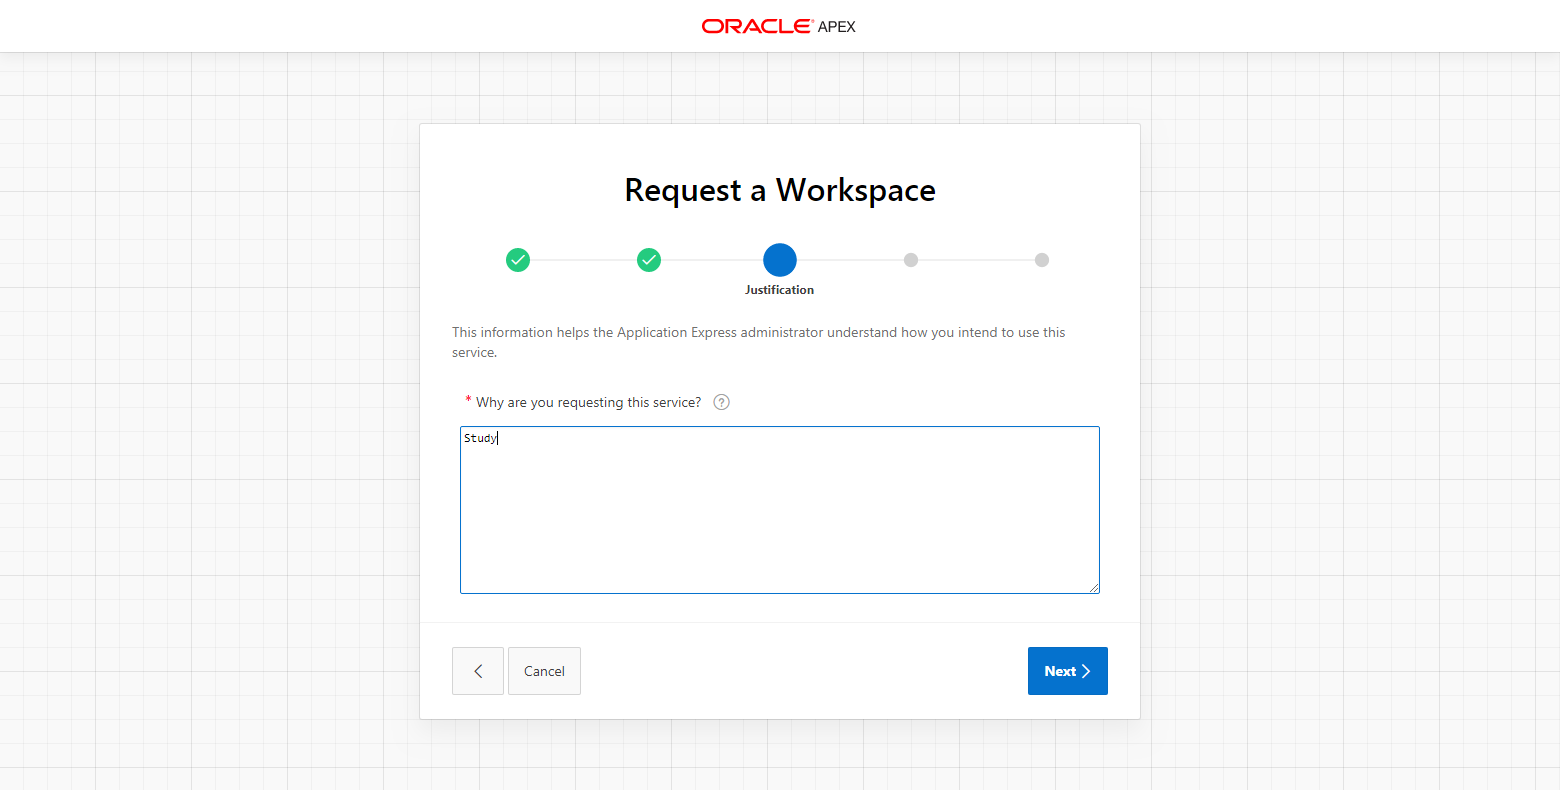
\includegraphics[scale=0.2]{figures/tahap4.png}
	\caption{\textit{Isi justification}}
	\end{center}	 
\end{figure}

\begin{figure}[!htbp]
\item[6] Ceklis pada kotak I accept the terms.
	\begin{center}
	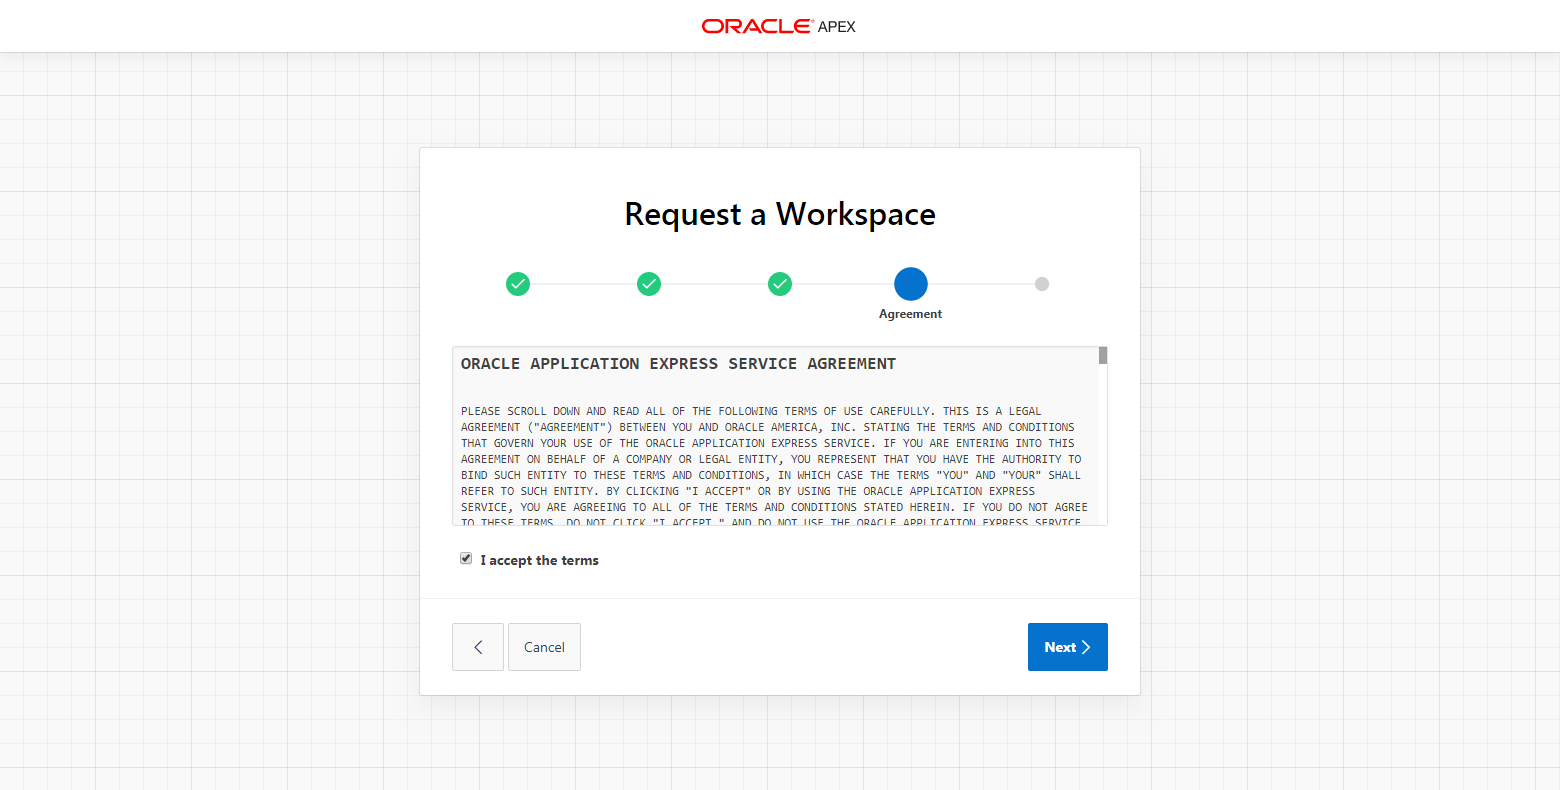
\includegraphics[scale=0.2]{figures/tahap5.png}
	\caption{\textit{Penanda agreement}}
	\end{center}	 
\end{figure}

\begin{figure}[!htbp]
\item[7] Setelah data benar, maka submit request.
	\begin{center}
	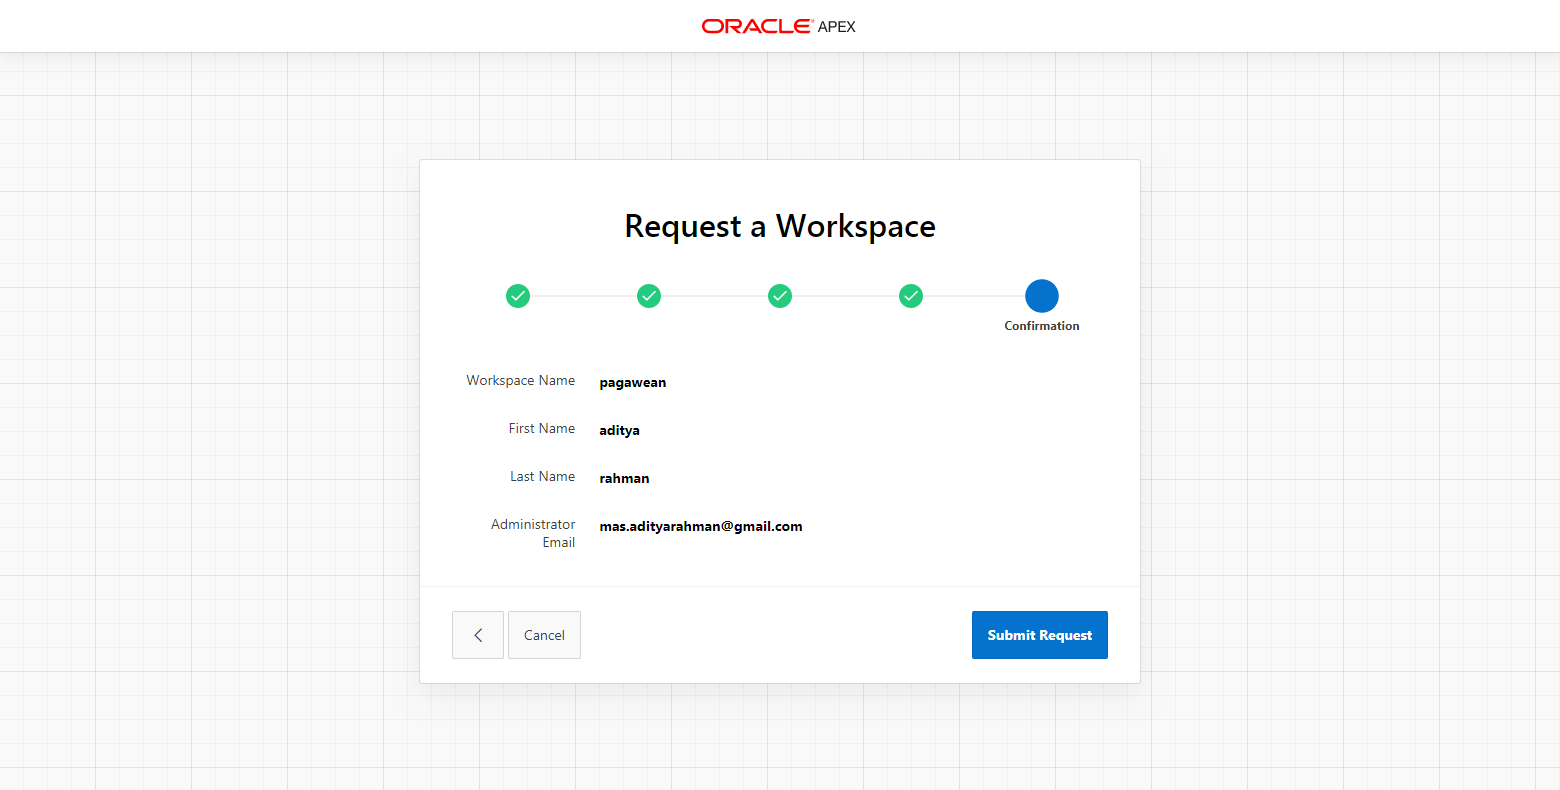
\includegraphics[scale=0.2]{figures/tahap6.png}
	\caption{\textit{klik submit request}}
	\end{center}	 
\end{figure}

\begin{figure}[!htbp]
\item[8] Maka selanjutnya cek email untuk melanjutkan ke tahap berikutnya.
	\begin{center}
	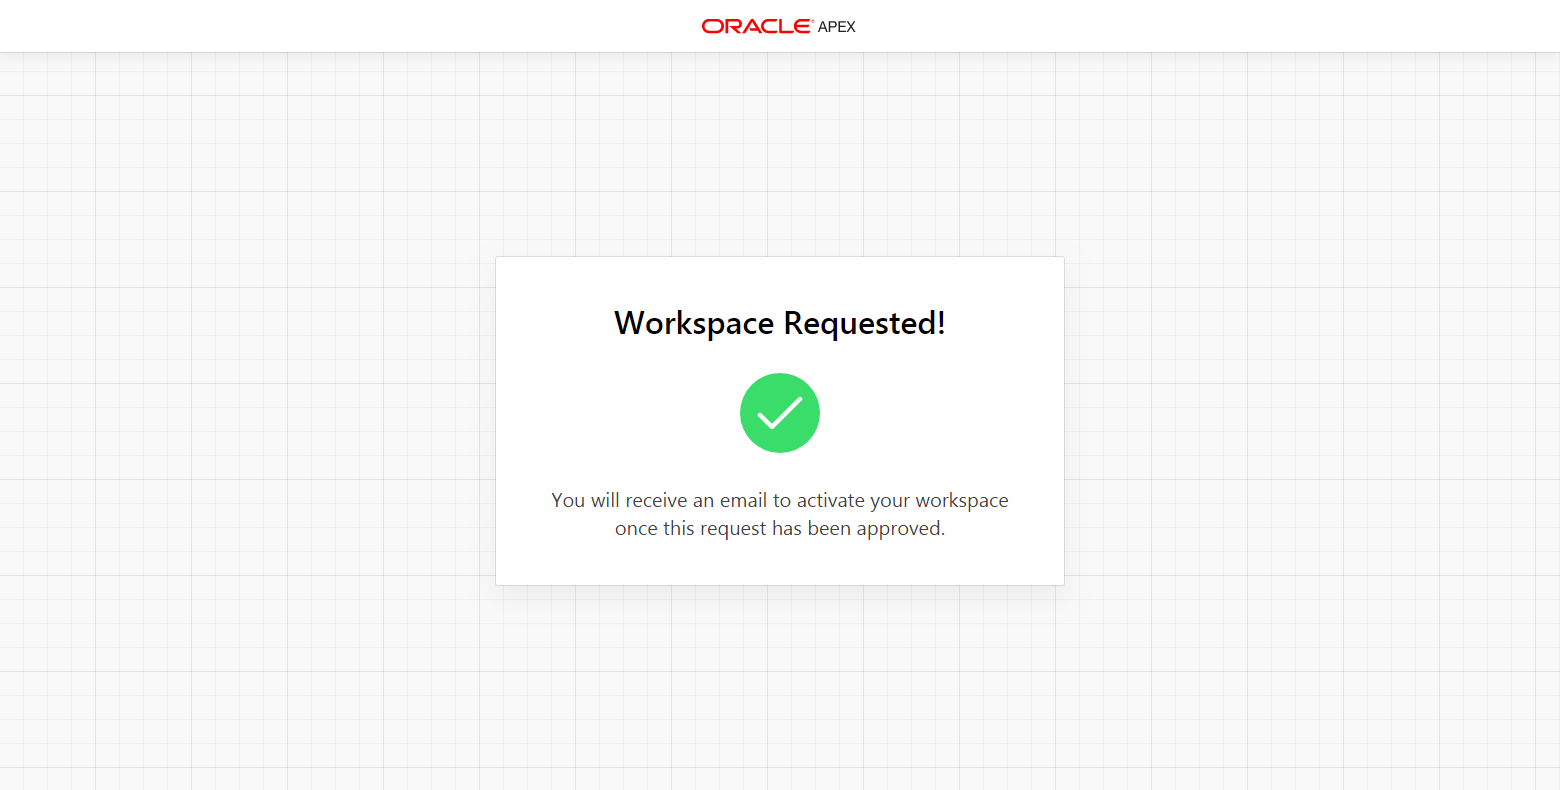
\includegraphics[scale=0.2]{figures/tahap7.png}
	\caption{\textit{Tampilan workspace requested}}
	\end{center}	 
\end{figure}

\begin{figure}[!htbp]
\item[9] Buka email, dan pilih create workspace
	\begin{center}
	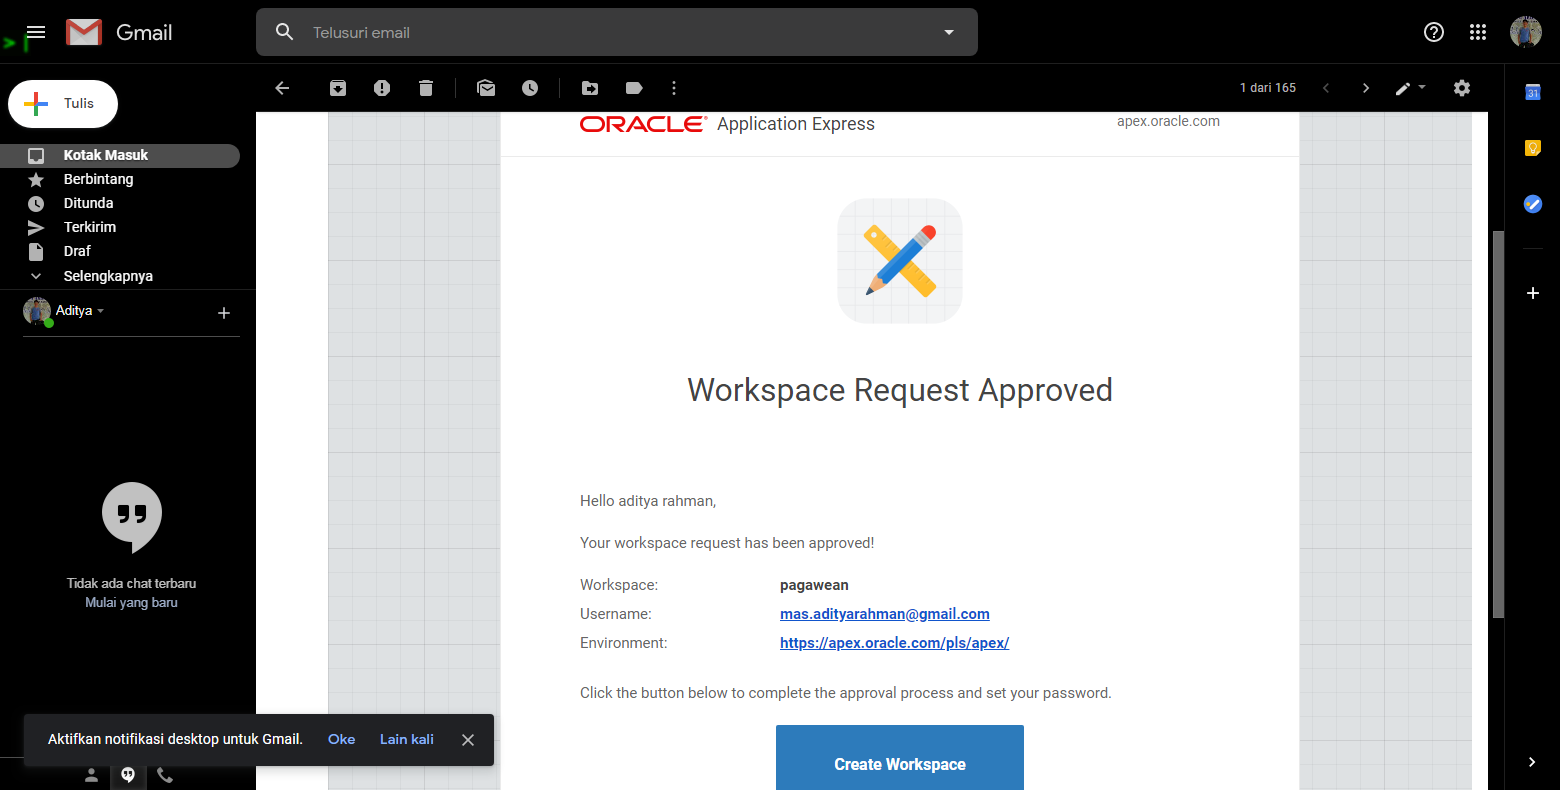
\includegraphics[scale=0.2]{figures/tahap8.png}
	\caption{\textit{Email dari oracle}}
	\end{center}	 
\end{figure}

\begin{figure}[!htbp]
\item[10] Maka akan diarahkan ke tampilan halaman sukses.
	\begin{center}
	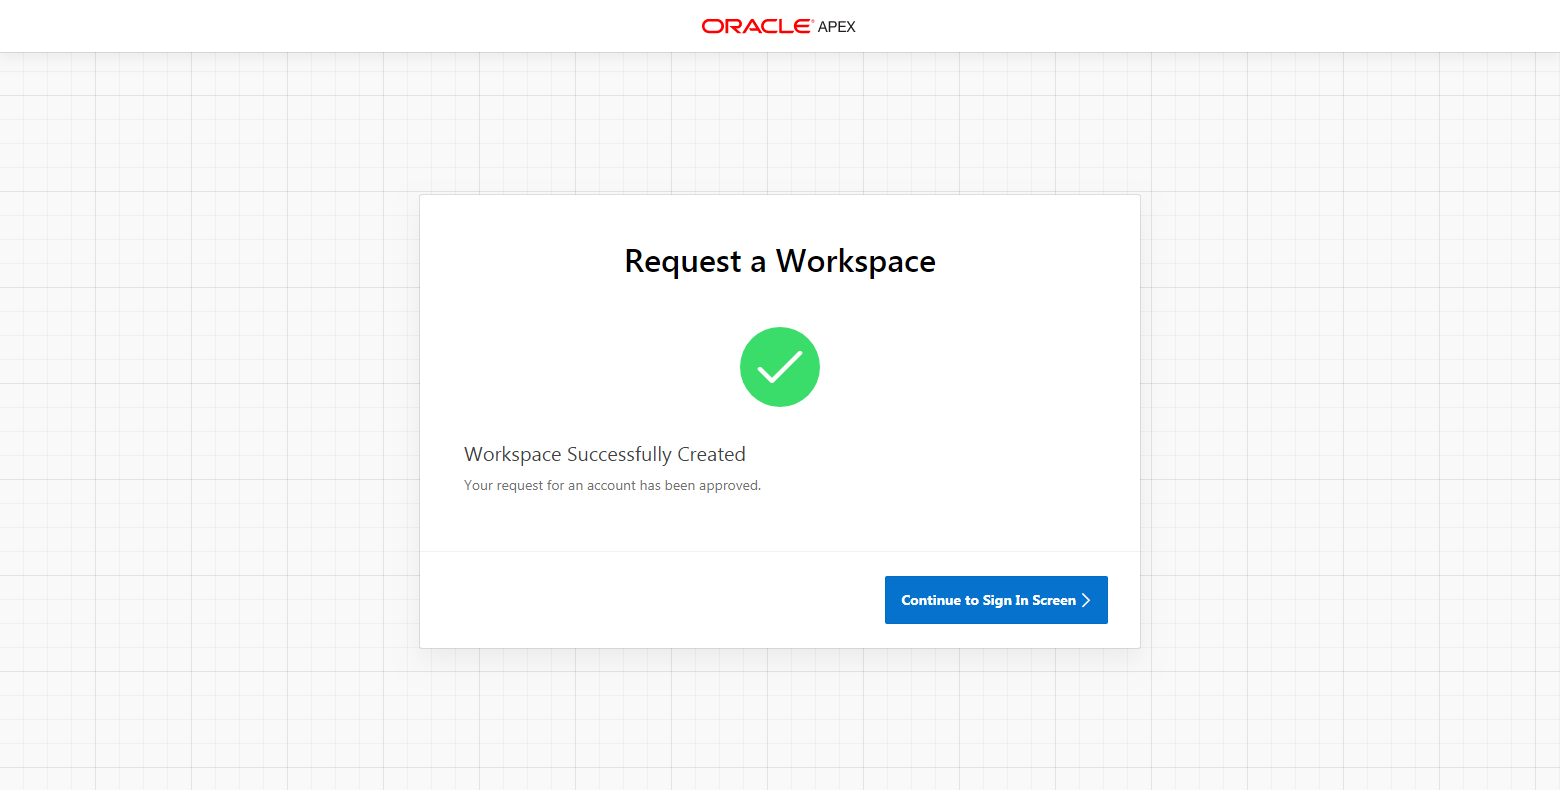
\includegraphics[scale=0.2]{figures/tahap9.png}
	\caption{\textit{Succes}}
	\end{center}	 
\end{figure}

\begin{figure}[!htbp]
\item[11] Maka setelah itu akan masuk ke tampilan beranda oracle apex
	\begin{center}
	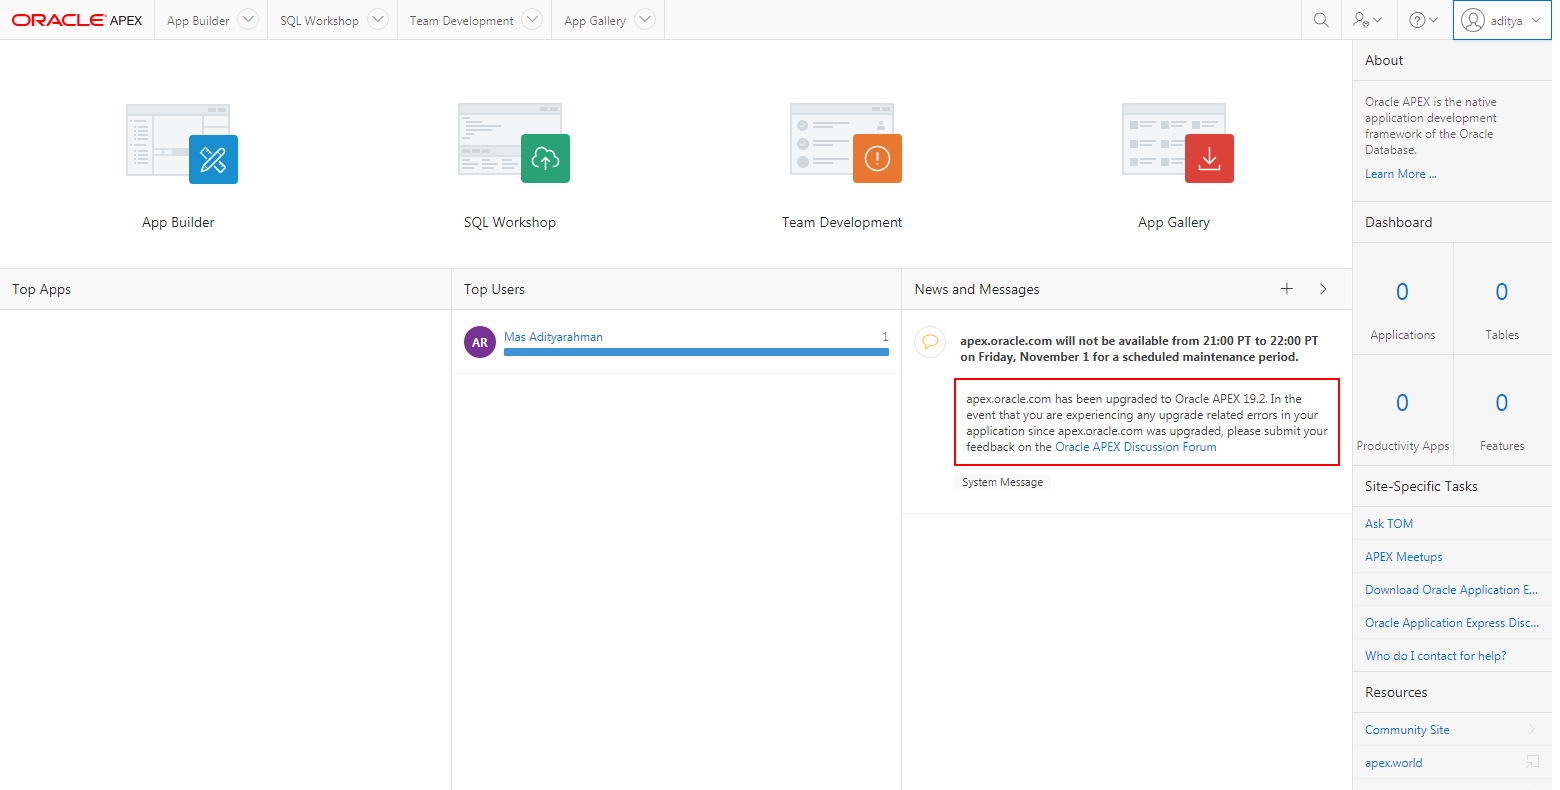
\includegraphics[scale=0.2]{figures/tahap10.png}
	\caption{\textit{Tampilan aplikasi oracle apex}}
	\end{center}	 
\end{figure}

\begin{figure}[!htbp]
\item[12] Pembuatan aplikasi oracle apex
	\begin{center}
	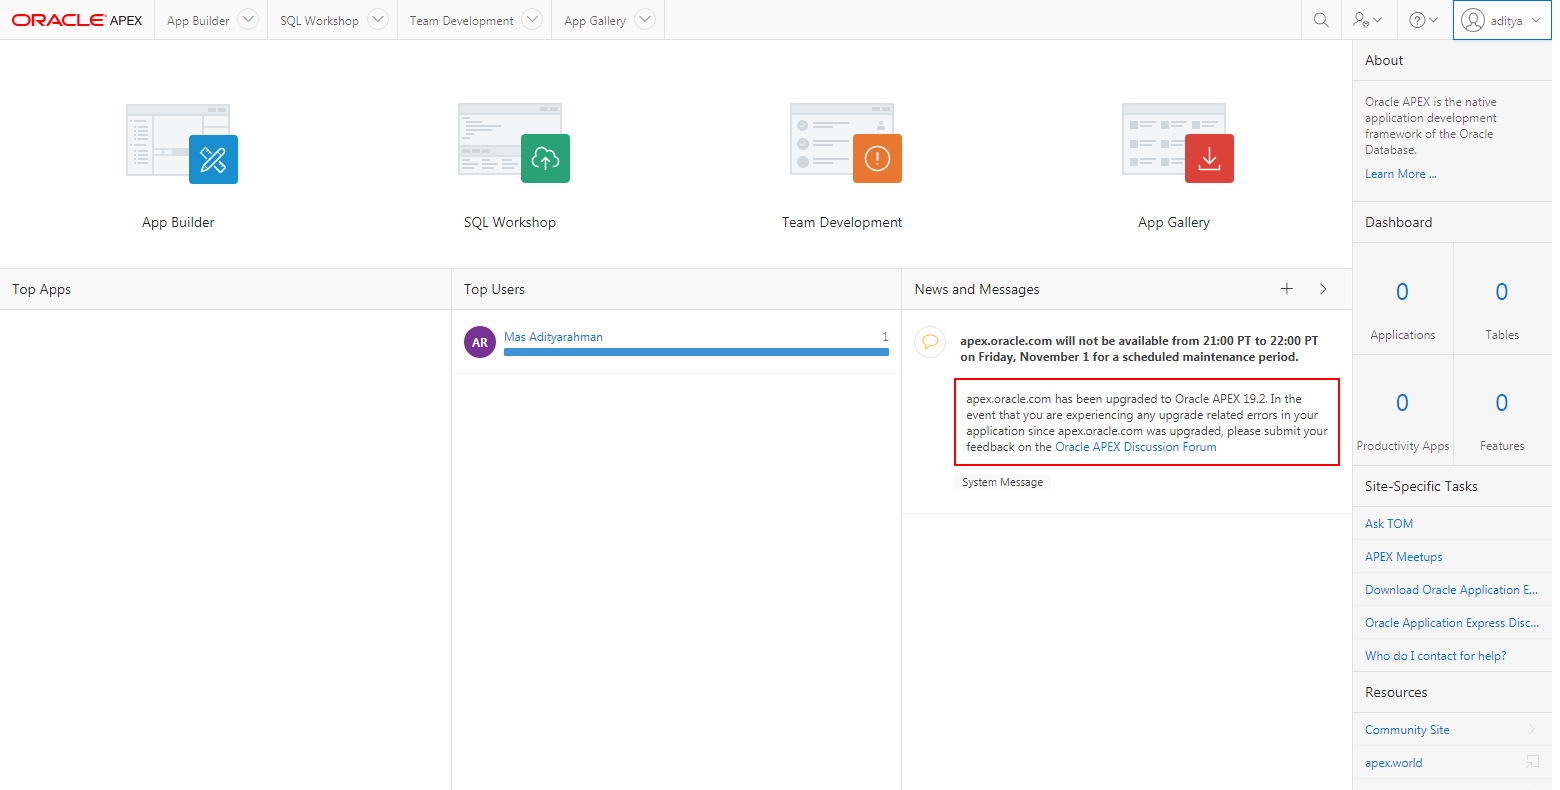
\includegraphics[scale=0.2]{figures/tahap10.png}
	\caption{\textit{Pilih app builder}}
	\end{center}	 
\end{figure}

\begin{figure}[!htbp]
\item[13] Maka akan masuk di tampilan create an application
	\begin{center}
	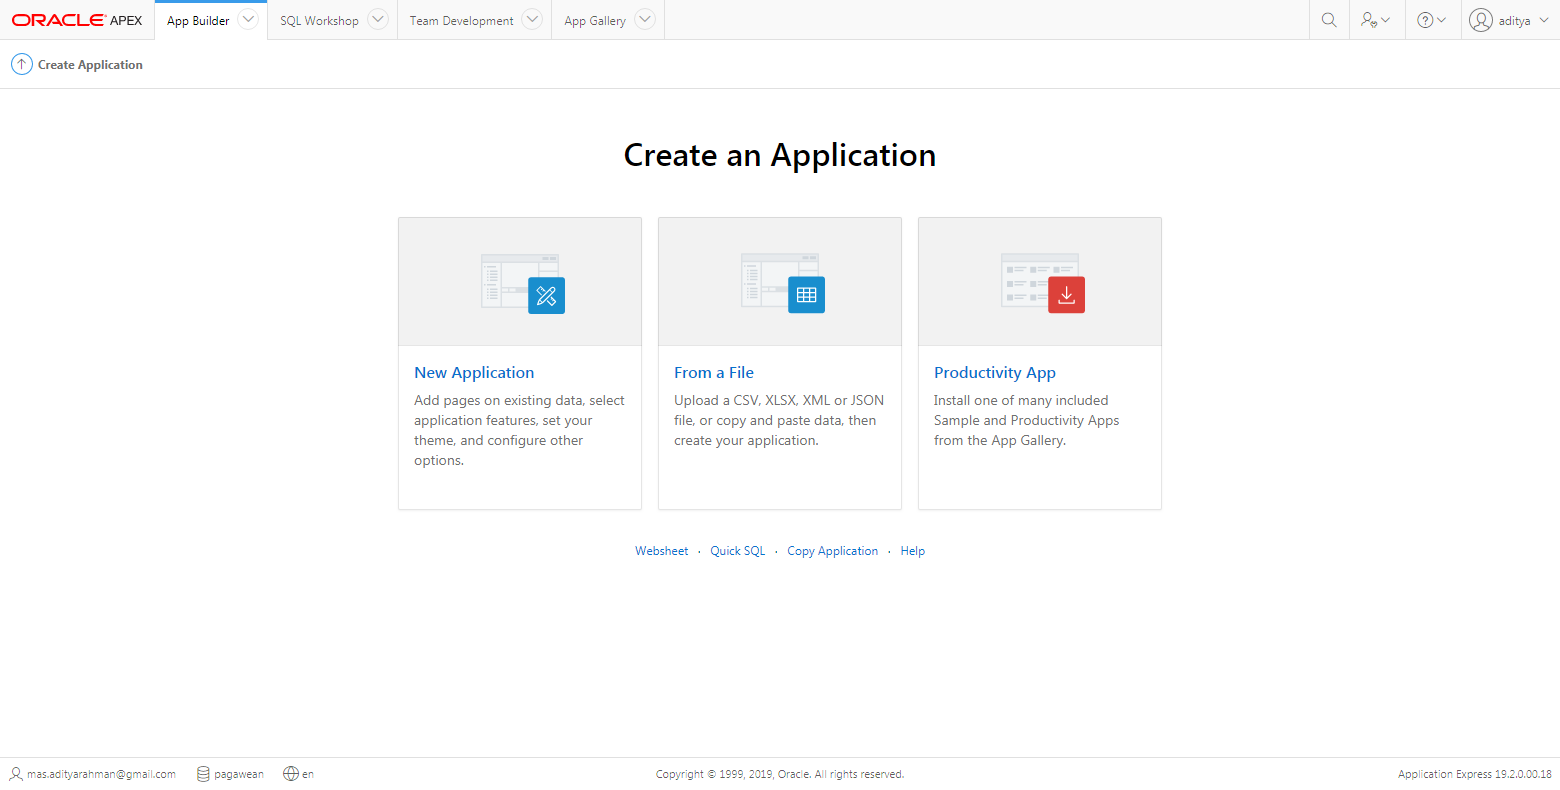
\includegraphics[scale=0.2]{figures/tahap12.png}
	\caption{\textit{Pilih from a file}}
	\end{center}	 
\end{figure}

\begin{figure}[!htbp]
\item[14] Drag and Drop file dengan format .csv
	\begin{center}
	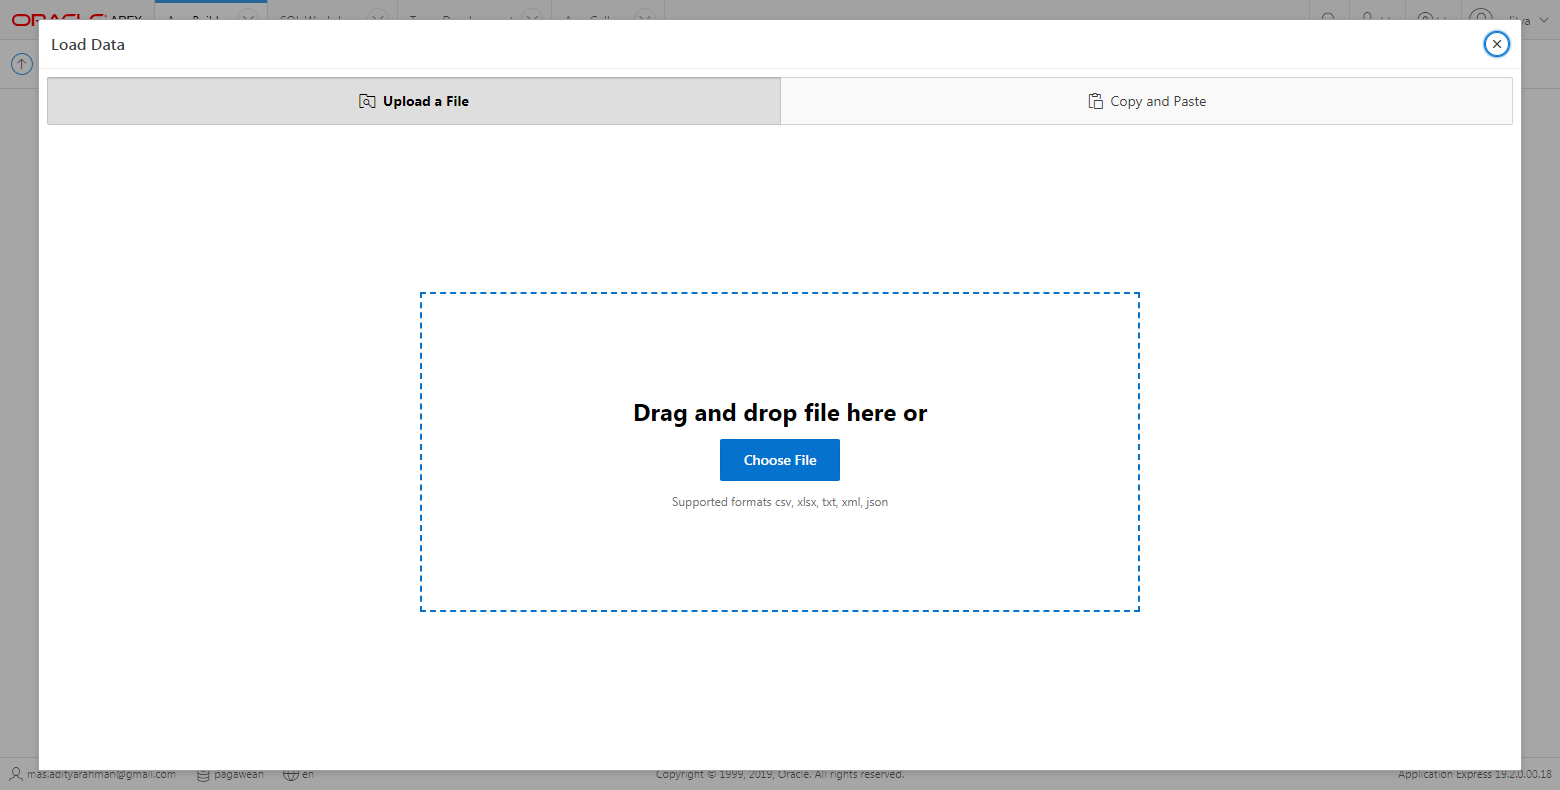
\includegraphics[scale=0.2]{figures/tahap13.png}
	\caption{\textit{drag and drop file}}
	\end{center}	 
\end{figure}

\begin{figure}[!htbp]
\item[15] Maka file dengan format .csv akan terupload di apex
	\begin{center}
	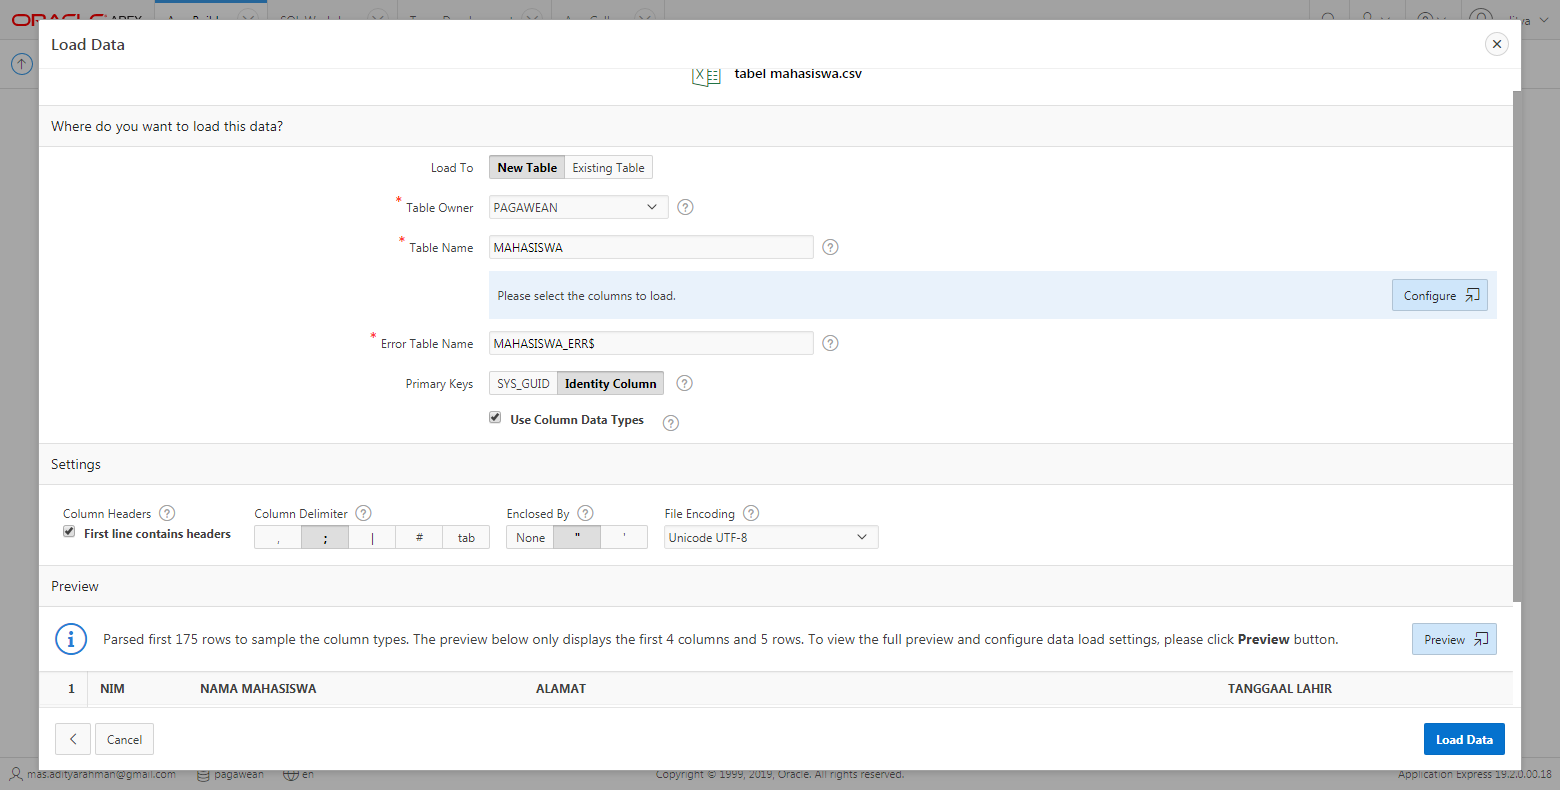
\includegraphics[scale=0.2]{figures/tahap14.png}
	\caption{\textit{File telah di upload}}
	\end{center}	 
\end{figure}

\begin{figure}[!htbp]
\item[16] Setelah file .csv berhasil di upload maka, pilih atau klik load data yang berada di pojok kanan bawah.
	\begin{center}
	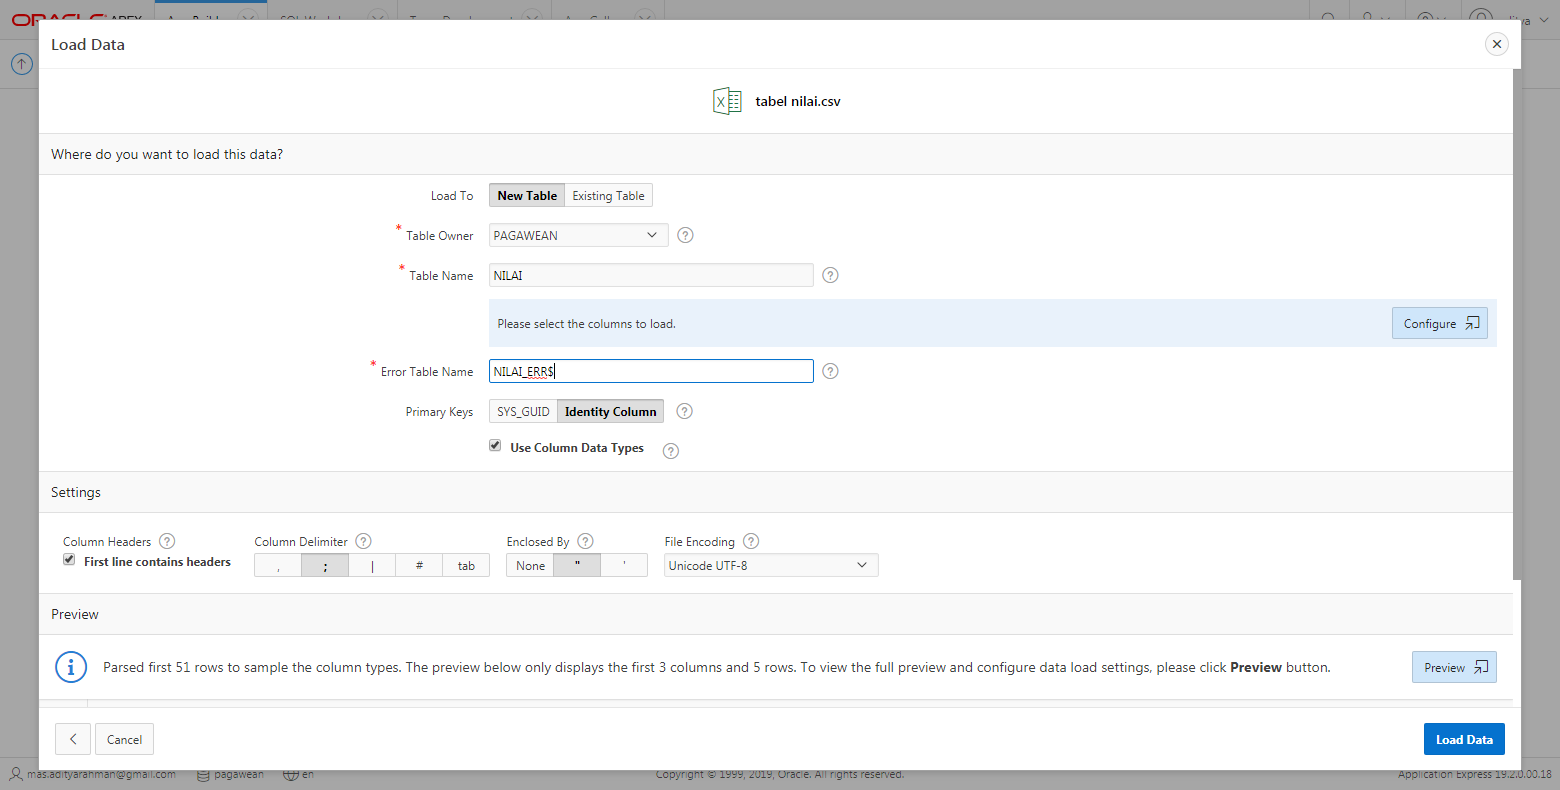
\includegraphics[scale=0.2]{figures/tahap18.png}
	\caption{\textit{Klik load data}}
	\end{center}	 
\end{figure}

\begin{figure}[!htbp]
\item[17] Setelah itu tambahkan halaman baru , dengan pilih add page.
	\begin{center}
	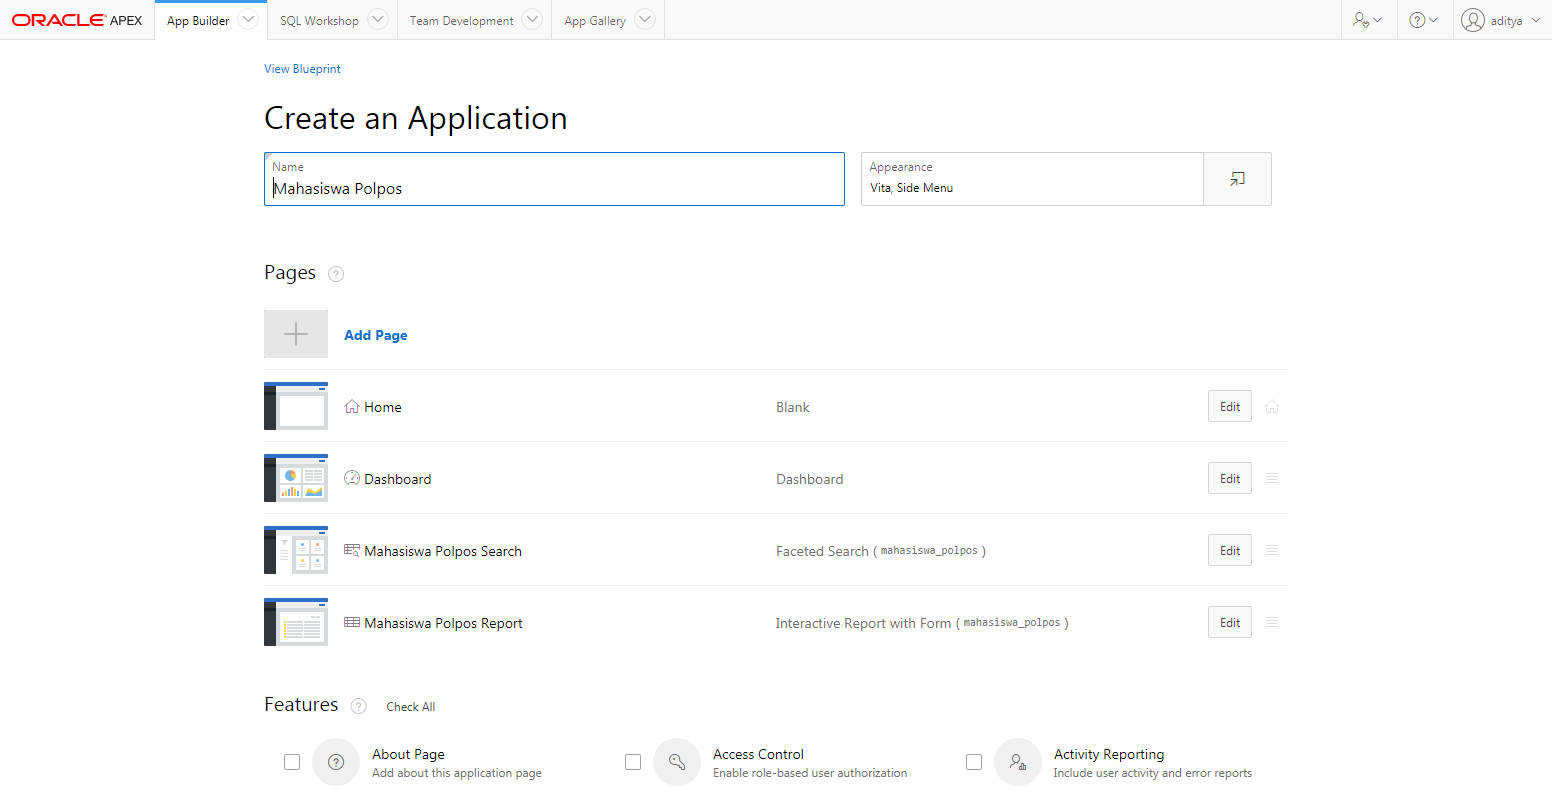
\includegraphics[scale=0.2]{figures/tahap19.png}
	\caption{\textit{Tambah add page}}
	\end{center}	 
\end{figure}

\begin{figure}[!htbp]
\item[18] Pilihlah interactive report
	\begin{center}
	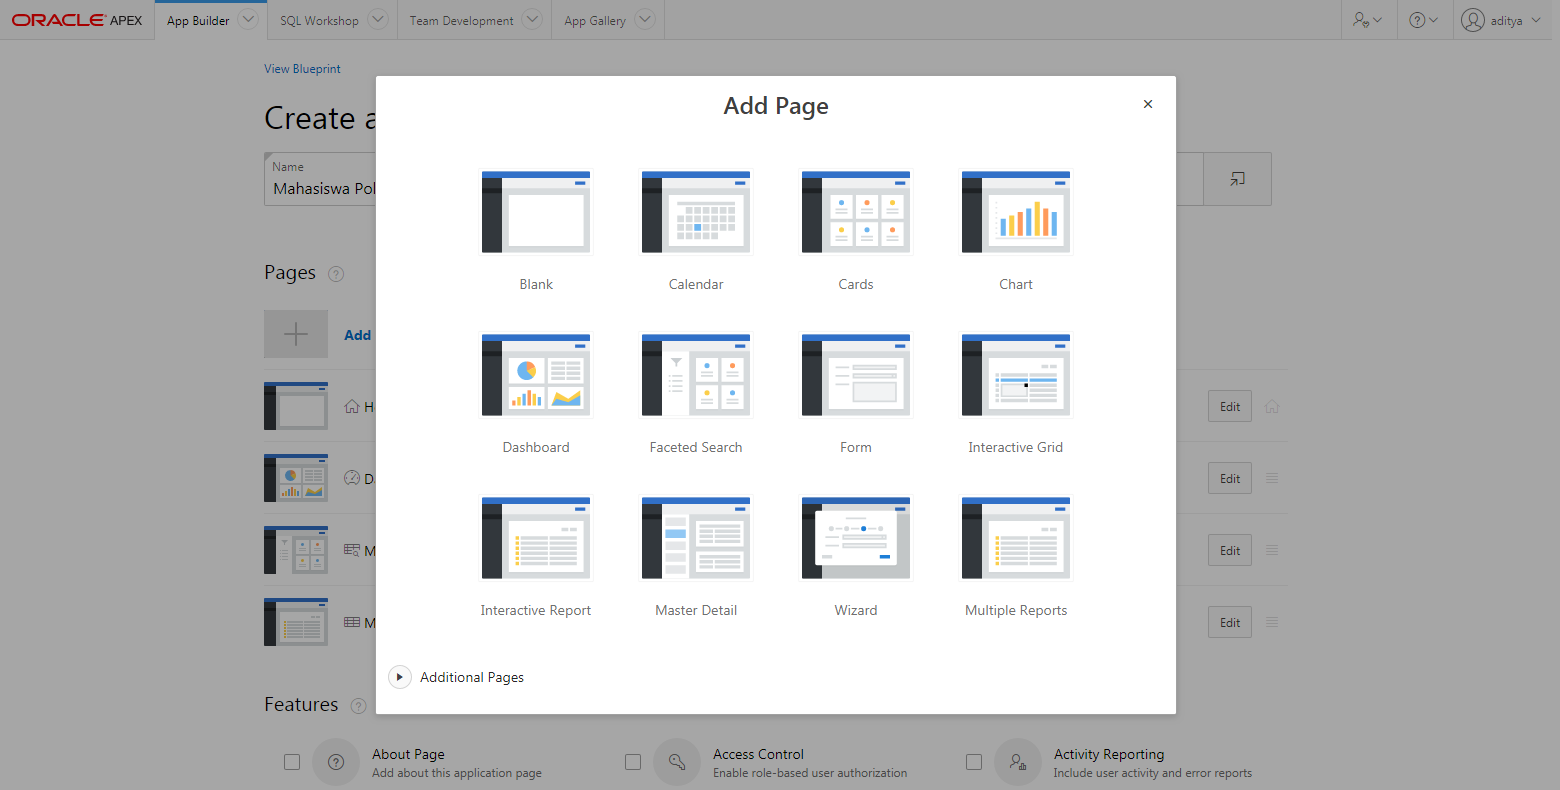
\includegraphics[scale=0.2]{figures/tahap20.png}
	\caption{\textit{Pilih interactive report}}
	\end{center}	 
\end{figure}

\begin{figure}[!htbp]
\item[19] Isi page name dan pilih tabel or view, setelah disii klik add page yang berada di kanan bawah. 
	\begin{center}
	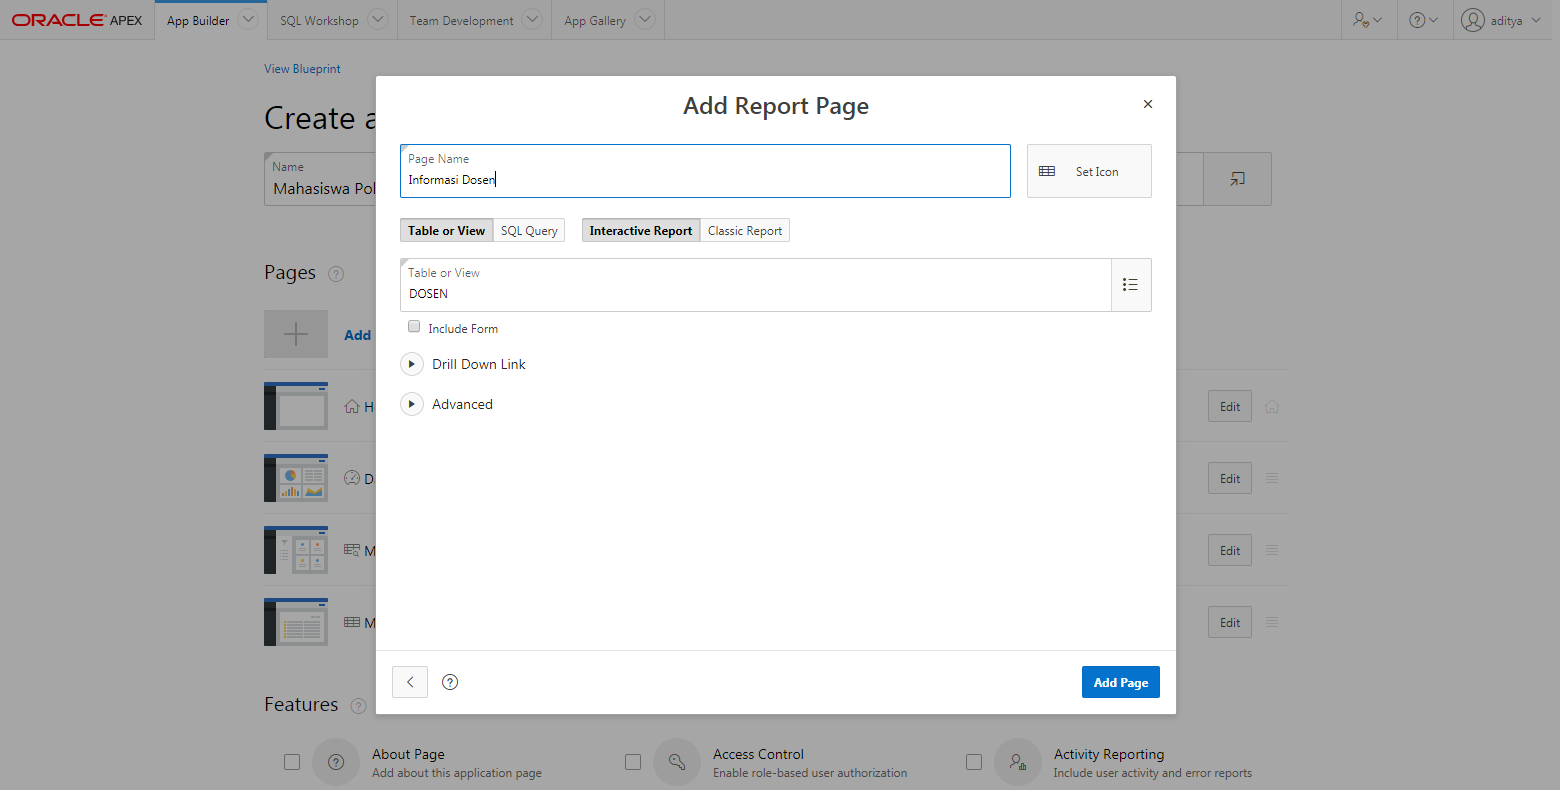
\includegraphics[scale=0.2]{figures/tahap21.png}
	\caption{\textit{Tahapan add report page}}
	\end{center}	 
\end{figure}

\begin{figure}[!htbp]
\item[20] Setelah diisi semua, klik create application
	\begin{center}
	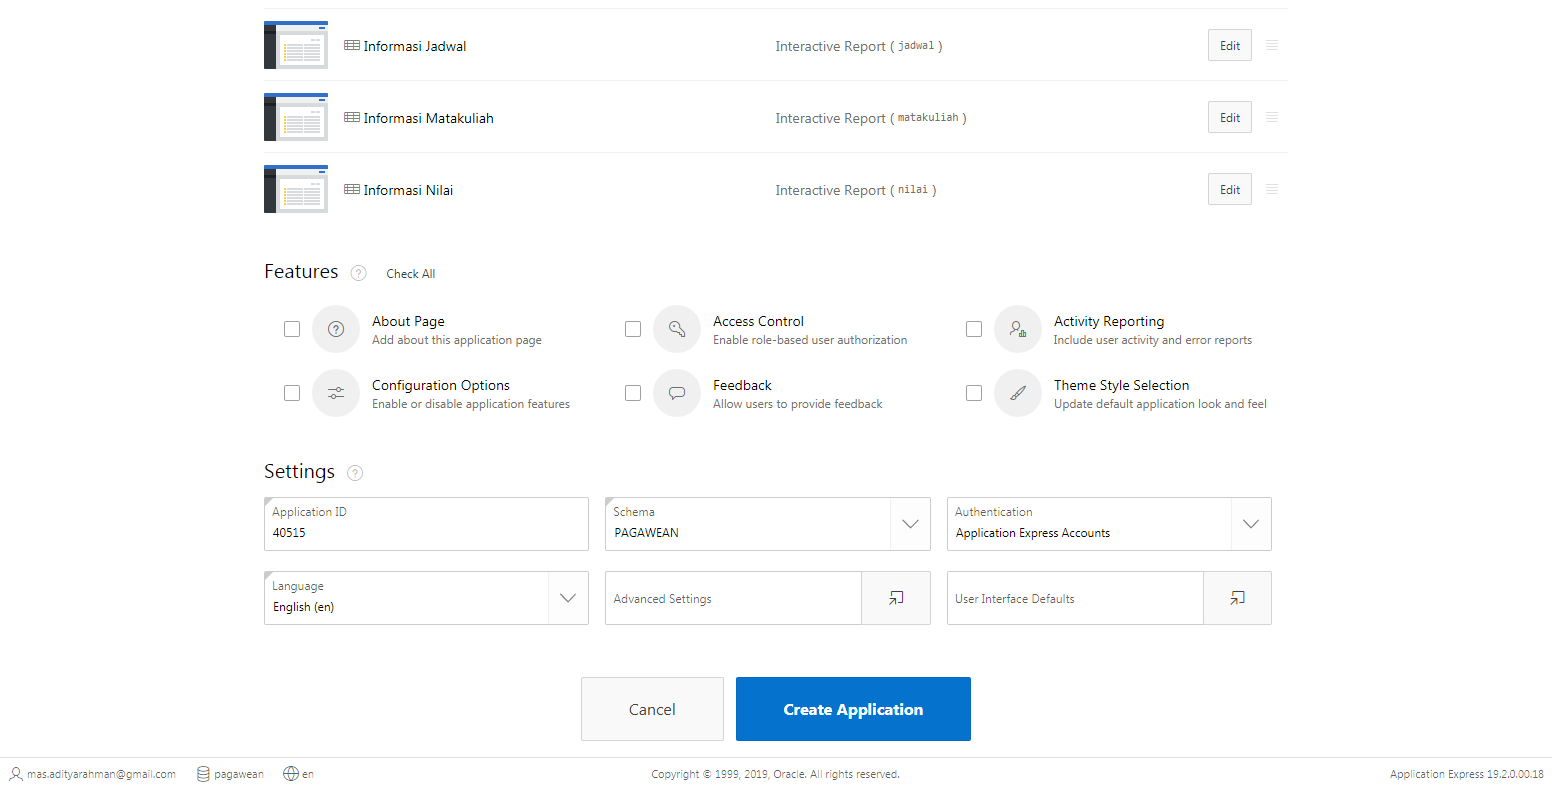
\includegraphics[scale=0.2]{figures/tahap22.png}
	\caption{\textit{pilih create application}}
	\end{center}	 
\end{figure}

\begin{figure}[!htbp]
\item[21]Tampilan Application telah berhasil dibuat, maka data-data telah dibuat melalui excel telah terupload didalam application apex.
	\begin{center}
	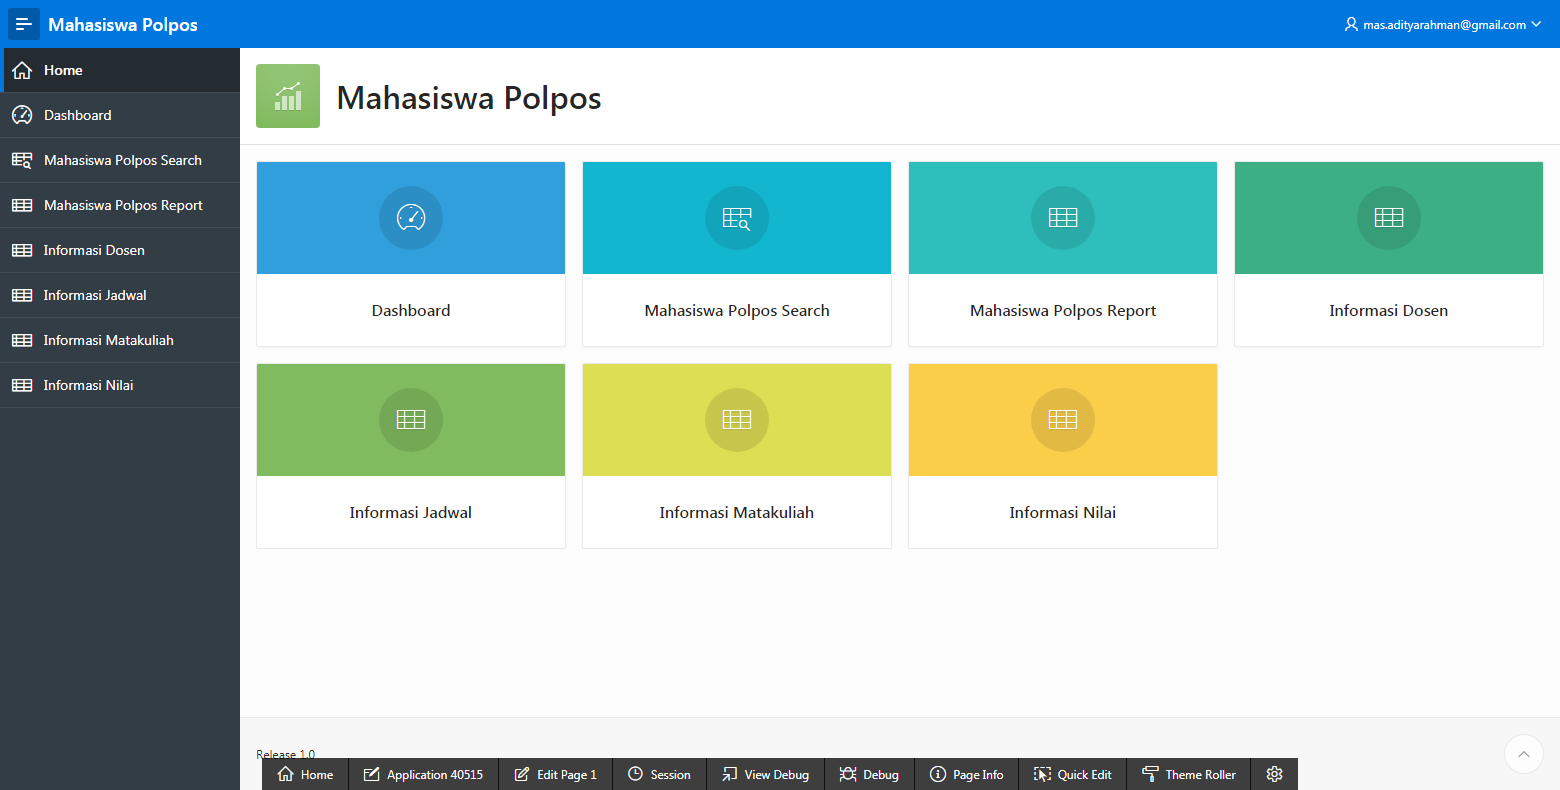
\includegraphics[scale=0.2]{figures/tahap23.png}
	\caption{\textit{Tampilan aplikasi}}
	\end{center}	 
\end{figure}

\begin{figure}[!htbp]
\item[22]Akun oracle apex yang telah dibuat \\
	\begin{center}
	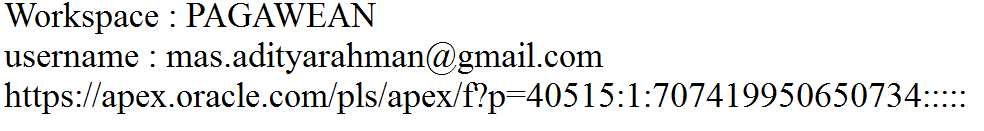
\includegraphics[scale=0.2]{figures/tahap24.png} \\
	https://apex.oracle.com/pls/apex/f?p=40515:1:707419950650734:::::
	\end{center}	 
\end{figure}
\end{enumerate}